\documentclass[12pt]{article}
\usepackage{xparse}
\usepackage[utf8]{inputenc}
\usepackage{graphicx}
\usepackage{amsmath}
\usepackage{calligra}



\usepackage{titlesec}
\titleformat{\section}[block]{\sffamily\Large\filcenter\bfseries}{\thesection.}{0.25cm}{\Large}
\titleformat{\subsection}[block]{\large\bfseries\sffamily}{\thesubsection.}{0.2cm}{\large}
\titleformat{\subsubsection}[block]{\small\sffamily}{\thesubsubsection}{0.18cm}{\large}


\usepackage{enumitem}
\DeclareMathAlphabet{\mathcalligra}{T1}{calligra}{m}{n}
\DeclareFontShape{T1}{calligra}{m}{n}{<->s*[2.2]callig15}{}
\newcommand{\scriptr}{\mathcalligra{r}\,}
\newcommand{\boldscriptr}{\pmb{\mathcalligra{r}}\,}
\usepackage{physics}
\newcommand{\ang}[1]{\langle #1 \rangle}
\usepackage{tcolorbox}
\usepackage{tikz}
\usepackage[a4paper]{geometry}
\usepackage{hyperref}
\title{\sffamily{PH 108 Formulae(Quiz 2)}}
\author{\sffamily{Advait Risbud}}
\date{May 21'}

\begin{document}
	\maketitle
	\sffamily
	
\newpage
\tableofcontents
\pagebreak
	\section{Mathematical Preliminaries}
	\begin{itemize}
		
		\item \textbf{Gradients}. 
		\begin{enumerate}
		\item Consider a scalar field T in 3-dimensions. If we move in the direction denoted by $\va{\textbf{dl}}$, then the change in the value of the scalar field T is denotes by 
		\begin{equation}
			dT=\grad{T}\vdot \va{\textbf{dl}}
		\end{equation}
	    \item Gradient gives the direction of largest increase in the value of the scalar field.
	\end{enumerate}
      
      
       \item \textbf{Properties of Grad, Div, and Curl}.
       \begin{enumerate}
       	\item $\grad{(f+g)}=\grad{f}+\grad{g}$
       	
       	\item $\grad \vdot (\va{A}+\va{B})=\grad \vdot \va{A}+\grad \vdot \va{B}$
       	
       	\item $\curl (\va{A}+\va{B})$ 
       	

       	
       	
       	\item $\grad{(kf)}=k(\grad{f}$)
       	
       	\item $\div{(k\va{A})}=k(\div{\va{A}})$
       	
       	\item $\curl (k\va{A})=k( \curl{\va{A}}$)
       	
       	\item $\grad{(fg)}=f(\grad{g})+g(\grad{f})$
       	
       	\item $\grad{(\va{A}\vdot \va{B})}=\va{A}\cross\curl{\va{B}}+\va{B}\cross \curl{\va{A}}+(\va{A}\vdot \grad)\va{B}+(\va{B}\vdot \grad)\va{A}$
       	
       	\item $\div{(f\va{A})}=f(\div{\va{A}})+\va{A}\vdot\grad{f}$
       	
       	\item $\div{\va{A}\cross\va{B}}=\va{B}\vdot(\curl{\va{A}})-\va{A}\vdot(\curl{\va{B}})$
       	
       	\item $\curl{(f\va{A}}=f(\curl{\va{A}})-\va{A}\cross\grad{f}$
       	
       	\item $\curl{(\va{A}\cross\va{B})}=(\va{B}\vdot\grad)\va{A}-(\va{A}\vdot\grad)\va{B}+\va{A}(\div{\va{B}})-\va{B}(\div{\va{A}})$
       \end{enumerate}
   \begin{tcolorbox}[colback=blue!5, colframe=blue!75!black, title=Double derivatives]
   	\begin{enumerate}
   		\item Divergence of the gradient(\textbf{laplacian}). $$\div (\grad{f})=\pdv[2]{f}{x}+\pdv[2]{f}{y}+\pdv[2]{f}{z}$$ We get the laplacian operator from here as follows, 
   		
   		\begin{align}
   			\laplacian&=\pdv[2]{}{x}+\pdv[2]{}{y}+\pdv[2]{}{z}
   		\end{align}
   		\item Curl of a gredient
   		\begin{align}
   			\curl{(\grad{f})}=0
   		\end{align}
   		\item Gradient of the divergence
   		\begin{align}
   			\grad{(\div{\va{A}})}
   		\end{align}
   		\item Divergence of a curl
   		\begin{align}
   			\div{(\curl{\va{A}})}=0
   		\end{align}
   		\item Curl of the curl
   		\begin{align}
   			\curl{(\curl{\va{A}})}=\grad{(\div{\va{A}})}-\laplacian{\va{A}}
   		\end{align}
   		\end{enumerate}
   \end{tcolorbox}
   \item \textbf{Co-ordinate systems}\\
   
   \begin{enumerate}
   	\item \textbf{Relations between magnitudes}\\
   	2-D: 
   	\begin{align}
   		x&=r\cos\phi \\
   		y&=r\sin\phi
   	\end{align}\\
   3-D: \\
   Spherical:\\
   \begin{align}
   	x&=r\sin\theta\cos\phi \\
   	y&=r\sin\theta\sin\phi \\
   	z&=r\cos\theta
   \end{align} \\

Cylindrical:\\
\begin{align}
	x&=s\cos \phi \\
	y&=s\sin \phi \\
	z&=z 
\end{align}
   
   \item \textbf{Unit vectors} \\
   In general, the unit vector is the direction of increase in that variable.\\
   2-D: 
   \begin{gather}
   	\begin{pmatrix}
   		\hat{r}\\
   		\hat{\theta}
   	\end{pmatrix}
   =
   \begin{pmatrix}
   	\cos\phi & \sin\phi \\
   	-\sin\phi& \cos\phi
   \end{pmatrix}
   \begin{pmatrix}
   	\hat{i}\\
   	\hat{j}
   \end{pmatrix}
   \end{gather}\\
3-D:\\
Spherical:\\
   \begin{gather}
   	\begin{pmatrix}
   		\hat{r}\\
   		\hat{\phi}\\
   		\hat{\theta}
   	\end{pmatrix}
   =
   \begin{pmatrix}
   	\sin\theta\cos\phi & \sin\theta\sin\phi & \cos\theta \\
   	-\sin\phi          & \cos\phi           & 0          \\
   	\cos\theta\cos\phi & \cos\theta\sin\phi & -\sin\theta  
   \end{pmatrix} 
\begin{pmatrix}
	\hat{i}\\
	\hat{j}\\
	\hat{k}
\end{pmatrix}
   \end{gather} \\
Cylindrical:\\
\begin{gather}
   	\begin{pmatrix}
	\hat{s}\\
	\hat{\phi}\\
	\hat{z}
\end{pmatrix}
=
\begin{pmatrix}
	\sin \phi & \cos \phi & 0 \\
	-\sin\phi & \cos\phi  & 0          \\
	0         & 0         & 1
\end{pmatrix} 
\begin{pmatrix}
	\hat{i}\\
	\hat{j}\\
	\hat{k}
\end{pmatrix}
\end{gather}

The polar co-ordinate system is orthogonal.
   \item \textbf{Distance elements}\\
   2-D: \begin{equation}
   	d\va{\textbf{l}}=dr\hat{r}+rd\theta\hat{\theta}
   \end{equation}\\
   3-D: \\
   Spherical:\\
   \begin{equation}
   	d\va{\textbf{l}}=dr\hat{r}+rd\theta\hat{\theta}+r\sin\theta d\phi \hat{\phi}
   \end{equation}
Cylindrical:\\
   \begin{equation}
   	d\va{\textbf{l}}=ds\hat{s}+sd\phi\hat{\phi}+ dz \hat{z}
   \end{equation}

   \end{enumerate}
\item \textbf{Operators in all co-ordinate systems}\\
Cartesian:\\
\begin{equation}
	\qq{Gradient:}\ \grad{\textbf{T}}=\bigg(\pdv{T}{x}\bigg)\hat{x}+\bigg(\pdv{T}{y}\bigg)\hat{y}+\bigg(\pdv{T}{z}\bigg)\hat{z}
\end{equation}\\
\begin{equation}
	\qq{Divergence:}\ \div{v}=\pdv{v_x}{x}+\pdv{v_y}{y}+\pdv{v_z}{z}
\end{equation}\\
\begin{equation}
	\qq{Curl:}\ \curl{v}=\bigg(\pdv{v_z}{y}-\pdv{v_y}{z}\bigg)\hat{x}+\bigg(\pdv{v_x}{z}-\pdv{v_z}{x}\bigg)+\bigg(\pdv{v_y}{x}-\pdv{v_x}{y}\bigg)
\end{equation}\\
\begin{equation}
	\qq{Laplacian:}\ \laplacian{v}=\pdv[2]{v_x}{x}+\pdv[2]{v_y}{y}+\pdv[2]{v_z}{z}
\end{equation}
Spherical:\\
\begin{figure}[h]
	\centering
	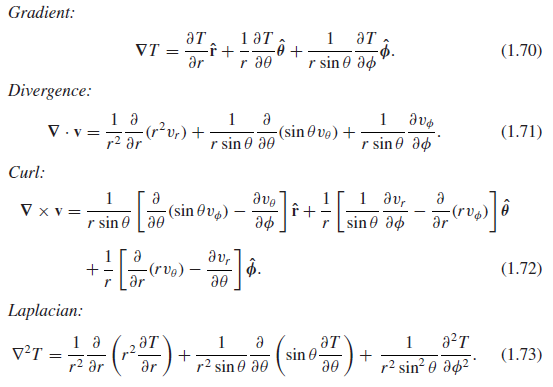
\includegraphics{./img/operators_spherical.png}
\end{figure}\\
Cylindrical:\\
\begin{figure}[h]
	\centering
	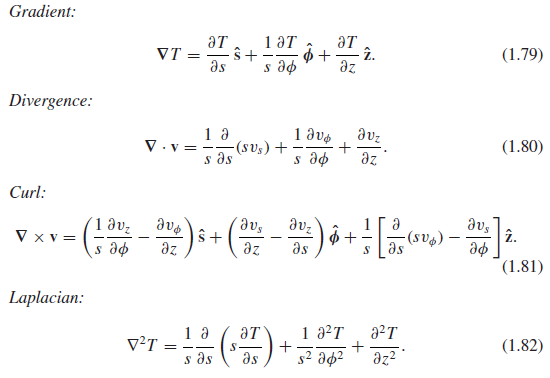
\includegraphics{./img/operators_cyl.png}
\end{figure}



\begin{tcolorbox}[colback=red!5,colframe=red!75!black,title=\textbf{Theorems of Vector Calculus}]
	\begin{enumerate}
		\item \textbf{FTOVC}
		\begin{equation}
			\int_{a}^{b}\grad{\va{v}}\cdot d\va{l}=\va{v}(b)-\va{v}(a)
		\end{equation}
		Corollary: 
		\begin{equation}
			\oint_C \grad{\va{v}}\cdot d\va{l}=0
		\end{equation}
		\item \textbf{Gauss's/Divergence Theorem} 
		\begin{equation}
		 \oint_S \va{v}\cdot \,d\va{a}=\int_V (\div{\va{v}})\, d\tau
		\end{equation}
	This states that the flux of a vector field $\va{v}$ through a closed surface $S$ is equal to the volume integral of the divergence of that field over the volume that $S$ encloses.
	
	\item \textbf{Stoke's Theorem}
	\begin{equation}
		\oint_{\delta S}\va{v}\cdot d\va{l}=\int_S (\curl{\va{v}})\cdot d\va{a}
	\end{equation}
Where $\delta S$ is the boundary of the surface $S$.
	\end{enumerate}
\end{tcolorbox}

\item \textbf{Dirac Delta Function}\\
1-D:\\
$$\delta (x-a)=
	\begin{cases}
		0, \text{ for } x\neq a \\
		\infty, \text{ for } x=a
	\end{cases}
$$\\
Integral of the delta function,
$$\int_{b}^{c}\delta(x-a)dx=
\begin{cases}
	1, \text{ for } b\leq a \leq c\\
	0, \text{ otherwise }
\end{cases}.
$$\\
\begin{equation}
	f(x)\delta(x-a)=f(a)\delta(x-a) \\
\end{equation}

Delta function picks out values as,

$$\int_{b}^{c}f(x)\delta(x-a)dx=
\begin{cases}
	f(a), \text{ for } b\leq a \leq c\\
	0, \text{ otherwise }
\end{cases}.
$$

2 delta functions $D_1(x)$ and $D_2(x)$ are considered equal(for all ordinary $f(x)$) if 
\begin{equation}
	\int_{-\infty}^{\infty}f(x)D_1(x)dx=\int_{-\infty}^{\infty}f(x)D_2(x)dx
\end{equation}
Important result:
\begin{equation}
	\delta(kx)=\frac{1}{\abs{k}}\delta(x) \\
\end{equation}

3-D:\\

Here \textbf{r} is the position vector.
\begin{equation}
	\delta^3(\va{r})=\delta(x)\delta(y)\delta(z)
\end{equation}
Analogous to the 1-D case,
\begin{equation}
	\int_{\text{all space}}\delta^3(\va{r})dx dy dz=1
\end{equation}

\begin{equation}
	\int_{\text{all space}}f(\va{r})\delta^3(\va{r}-\va{a})dx dy dz=f(\va{a}).
\end{equation}\\
Also, 
\begin{equation}
	\int_V f(\va{r})\delta^3(\va{r}-\va{a})dx dy dz= 
	\begin{cases}
		f(\va{a}), \text{ if } \va{a}\in V\\
		0,\text{ if } \va{a} \not\in V
	\end{cases}
\end{equation}
Important:
\begin{equation}
	\div{(\frac{\hat{r}}{r^2})}=4\pi\delta^3(\va{r}) 
\end{equation}

\item \textbf{Helmholtz' Theorem}\\
 Consider a vector field $\vec{F}(\va{r})$ which satisfies:
 \begin{enumerate}
 	\item $\div{\vec{F}}=D(\va{r})$
 	\item $\curl{\vec{F}}=\vec{C}(\va{r})$
 	\item $\div{\vec{C}}=0$
 	\item Diminishes to zero as $\va{r}\to\infty$
 \end{enumerate}
Then we can write the field as the sum of divergence-free(solenoidal) and curl-free(irrotational) fields as follows,
\begin{equation}
	\vec{F}(\va{r})=-\grad{U(\va{r})}+\curl{\vec{W}(\va{r})}
\end{equation} 
where $U(\va{r})$ and $\vec{W}(\va{r})$ are the scalar and vector potentials respectively, and are given by
\begin{align}
	      U(\va{r})&=\frac{1}{4\pi}\int \dfrac{D(\va{r'})}{\abs{\va{r}-\va{r'}}}d\tau'  \\
	\vec{W}(\va{r})&=\frac{1}{4\pi}\int \dfrac{\vec{C}(\va{r'})}{\abs{\va{r}-\va{r'}}}d\tau' .
\end{align}
Note: integrals are w.r.t $\va{r'}$ where $\va{r'}$ is the location of the source/sink of the field and differential operators are w.r.t $\va{r}$ where $\va{r}$ is the location where field/potential is to be calculated. 
	\end{itemize}

\section{Electrostatics}
\begin{itemize}
\item	Maxwell's equations for electrostatic fields:
	\begin{equation}
		\div{\vec{E}}=\frac{\rho(\va{r})}{\epsilon_0}
	\end{equation}
	
	\begin{equation}
		\curl{\vec{E}}=0
	\end{equation}

\item Couloumb's law:
\begin{equation}
	\vec{E}(\va{r})=\dfrac{1}{4\pi\epsilon_0}\int\dfrac{\rho(\va{r'})}{ \scriptr^2}\hat{\hat{\scriptr}}d\tau'
\end{equation}

Where {\large $\va{\scriptr}=\va{r}-\va{r'}$} is the separation vector between the source charge(at $\va{r'}$) to where the field is being calculated($\va{r}$).

\item Electrostatic potential:
\begin{equation}
	V(\va{r})=\frac{1}{4\pi \epsilon_0}\int \frac{\rho(\va{r'})}{\abs{\va{r}-\va{r'}}}d\tau'\label{43}
\end{equation}
Poisson's equation: 
\begin{equation}
	\laplacian{V}=-\frac{\rho(\va{r})}{\epsilon_0}
\end{equation}
In regions of zero charge density we get Laplace's equation:
\begin{equation}
	\laplacian{V}=0
\end{equation}

\subsection{ Boundary Conditions:}

\begin{tcolorbox}
	\begin{itemize}
		\item Gauss's Law: 
		\begin{equation}
			\oint \va{E}\cdot d\va{a}=\frac{Q_{en}}{\epsilon_0}
		\end{equation}
		
		\item BCs for fields:
		\begin{align}
		E^{\perp}_{above}-E^{\perp}_{below}&=\frac{\sigma}{\epsilon_0} \\
		              E^{\parallel}_{above}&=E^{\parallel}_{below} \\
		      \va{E}_{above}-\va{E}_{below}&=\frac{\sigma}{\epsilon_0}\vu{n}
	\end{align} 
		 \item Potential BCs:
		 \begin{equation}
		 	V_{above}=V_{below}\\
		 \end{equation}
	
	     \begin{align}
	     	E^{\perp}&=-\va{E}\cdot\vu{n}\\
	     	         &=-\grad{V}\cdot \vu{n}\\
	     	         &=-\pdv{V}{\textbf{n}}
	     \end{align} 
	 
	\end{itemize}
	\end{tcolorbox}
\subsection{General Formulae}
\item Energy density: \\
Here W=work done in assembling charges in this configuration. 
\begin{equation}
	W=\int \frac{1}{2} \epsilon E^2 d\tau
\end{equation}
Where $u_E$=energy density of the field,
\begin{equation}
	u_E=\frac{1}{2}\epsilon E^2
\end{equation}

\item Field at the surface of a conductor: 
\begin{equation}
	\va{E}=\frac{\sigma}{\epsilon_0}\vu{n}
\end{equation}

\item Electrostatic pressure:\\

\begin{equation}
	P=\frac{\sigma^2}{2\epsilon_0}
\end{equation}
\item Capacitance
\begin{itemize}
	\item $$Q=CV$$
	
	\item Capacitance of a spherical conductor of radius $R$:
	$$C=4\pi \epsilon_0 R $$
\end{itemize}

\end{itemize}

\section{Potentials}

\subsection{Solutions to LE:}

	\begin{enumerate}
		
		\item In 1-D:\\
		\begin{align}
			\dv[2]{V(x)}{x}&=0 \\
			           V(x)&=mx+c\\
			  \implies V(x)&=\frac{1}{2}\big[V(x+a)+V(x-a)\big]
		\end{align}
		The last equation allows us to conclude that there can be no maximum or minimum within the region of interest i.e. the domain of $x$. \\
		
		\item In 2-D:\\
		\begin{align}
			\pdv[2]{V}{x}+\pdv[2]{V}{y}&=0 \\
			                     V(x,y)&=\dfrac{1}{2\pi R}\oint_C V(x,y) dl
        \end{align}
		Again there can be no maxima or minima in the domain of interest, only at the boundary.
		
		\item In 3-D:\\
		Let the domain under consideration be a region of volume $V$ enclosed by a surface of area $S$.
		\begin{align}
			\pdv[2]{V}{x}+\pdv[2]{V}{y}+\pdv[2]{V}{z}&=0 \\
                                             V(x,y,z)&=\dfrac{1}{4\pi R^2}\oint_{S}V(x,y,z) da \qq{(S is a sphere here)}
		\end{align}

	No maxima or minima can exist in this volume. Earnshaw's theorem follows from this fact as no charge configuration can give a potential distribution with a point of stable equilibrium hence a charged particle cannot be trapped by other fixed charges.
	\end{enumerate}

\subsection{Uniqueness theorems}
\begin{tcolorbox}[colback=green!5, colframe=green!75!black, title=Theorems]
	\begin{enumerate}
		\item First uniqueness theorem: The solution to LE in some volume $V$ is uniquely determined if the potential is specified on the boundary surface.\\
		
		\item Second uniqueness theorem: In a volume $V$ surrounded by conductors and containing a specified charge density $\rho$, the electric field is uniquely determined if the total charge on each conductor is given.
	\end{enumerate}
\end{tcolorbox}

The domain definition means that the conductors are not a part of the domain and the charge density is specified everywhere else(see diagram in Griffiths). 

\subsection{Method of Images}
\begin{itemize}
	\item Image charge replicates potential distribution due to conducting surface.
	\item Image charge cannot be in the region where original charge is present.
	\item Image of image charge must be taken if mutiple surfaces are present.
	\item Combination of image charge and original charge gives potential distribution in region due to equivalent conducting plane and charge.
	\item Energy of infinite conducting sheet and charge '$q$'. 
	\begin{equation}
		U=\frac{1}{2}\bigg(-\dfrac{kq^2}{2d}\bigg)
	\end{equation}
	 
\end{itemize}

\subsection{Separations of Variables(Cartesian)}\label{cart SoV}
 The laplacian in cartesian co-ordinates is
\begin{equation}
	\pdv[2]{V}{x}+\pdv[2]{V}{y}+\pdv[2]{V}{z}=0 \label{eq:a}
\end{equation}
We take 
\begin{gather}
	V(x,y,z)=X(x)Y(y)Z(z) \qq{hence \eqref{eq:a} becomes} \\
	\frac{1}{X}\pdv[2]{X}{x}+\frac{1}{Y}\pdv[2]{Y}{y}+\frac{1}{Z}\pdv[2]{Z}{z}=0
\end{gather}
Since all three terms are in independent variables, each of them must be a constant such that their sum always equals zero. If variation is in all three directions i.e. none of the 3 terms are zero then the positive one can be taken as $k^2+l^2$ and in case of 2-D variation the positive one can be taken as $k^2$. \\

Which derivative should be taken positive and which negative is best seen through examples in Griffiths or tutorials. Some mathematical ideas however are important. 

\subsubsection{Common solutions of DEs}
\begin{enumerate}[label=\roman*]
	\item  
	\begin{align}
		   \frac{1}{X}\dv[2]{X}{x}&=k^2 \\
		\implies X(x)&=Ae^{kx}+Be^{-kx}
	    \end{align}
    \item 
    \begin{align}
    	\frac{1}{X}\dv[2]{V}{x}&=-k^2 \\
    	X(x)&=A\sin(kx)+B\cos(kx)
    \end{align}
    \item Hyperbolic trig functions:
    \begin{enumerate}[label=\alph*]
    \item  	$\sinh(x)=\dfrac{e^{x}-e^{-x}}{2}$
    \item   $\cosh(x)=\dfrac{e^{x}+e^{-x}}{2}$
    \end{enumerate}
\end{enumerate}


\subsubsection{Fourier's trick}\label{fourier}
As far as sinusoidal functions are concerned the trick involves finding the coefficients of a fourier series using orthgonality of the sine functions. If
\begin{align}
	V(y)&=\sum_{n=1}^{\infty}C_n\sin(\dfrac{n\pi y}{a}) \qq{we get,}\\
	\int_{0}^{a}V(y)\sin(\dfrac{n'\pi y}{a})dy&=\sum_{n=1}^{\infty}C_n\int_{0}^{a}\sin(\dfrac{n\pi y}{a})\sin(\dfrac{n' \pi y}{a})dy
\end{align}
From the orthogonality of the sine function we have

\begin{equation}
	\int_{0}^{a}\sin(\dfrac{n' \pi y}{a})\sin(\dfrac{n\pi y}{a})=\begin{cases}
		0  \quad &\text{if} \ n'\neq n\\
		\frac{a}{2} \quad &\text{if} \ n'=n \\
	\end{cases}
\end{equation}
So basically if we want the $n^{th}$ coefficient of the sine series then we should just multiply by the $n^{th}$ sine function to both sides and integrate within the limits of the variable. Here I have taken the boundaries to be at 0 and $a$ because that is the principal range for $\cos(\frac{n\pi y}{a})$(the choice of $V(y)$ and sine functions is all inspired by the topic at hand).

\subsection{Separation of Variables(Spherical Polar)}\label{polar SoV}
The laplacian in spherical co-ordinates is:
\begin{equation}
	\frac{1}{r^2} \pdv{r}(r^2 \pdv{V}{r}) + \dfrac{1}{r^2 \sin(\theta)} \pdv{\theta}\Big(\sin\theta \pdv{V}{\theta}\Big) + \dfrac{1}{r^2 \sin[2](\theta)}\pdv[2]{V}{\phi} =0
\end{equation}
while considering problems with azimuthal symmetry the equation reduces to:
\begin{equation}
	\frac{1}{r^2} \pdv{r}(r^2 \pdv{V}{r}) + \dfrac{1}{r^2 \sin(\theta)} \pdv{\theta}\Big(\sin\theta \pdv{V}{\theta}\Big)=0
\end{equation}
Once again we substitute $V$ as $V(r,\theta)=R(r)P(\theta)$ and divide the laplacian by V to get:
\begin{equation}
	\frac{1}{R}\pdv{r}\Bigg(r^2\pdv{R}{r}\Bigg) + \frac{1}{P \sin(\theta)}\pdv{\theta}(\sin(\theta)\pdv{P}{\theta})=0
\end{equation}

\subsubsection{Solution to radial part}
\begin{equation}
	R(r)=A_l r^l+\dfrac{B_l}{r^{l+1}}
\end{equation}

\subsubsection{Solution to polar part}
\begin{equation}
	P(\theta)=P_l(\cos\theta)
\end{equation}
Here $P_l(\cos\theta)$ is the $l^{th}$ Legendre Polynomial. These can be found using Rodrgiues' Formula:
\begin{equation}
	P_l(x)=\dfrac{1}{2^l l!}\dv[l]{(x^2-1)^l}{x} \qq{where $x=\cos\theta$}
\end{equation}

Some of them are:
\begin{align*}
	P_0(x)&=1\\
	P_1(x)&=x \\
	P_2(x)&=\dfrac{3x^2-1}{2}\\
	P_3(x)&=\dfrac{5x^3-3x}{2}
\end{align*}

Legendre polynomials are also orthogonal and \nameref{fourier} is applicable here as well. 
\begin{align}
	\int_{-1}^{1}P_l(x)P_{l'}(x)dx&=\int_{0}^{\pi}P_l(\cos\theta)P_{l'}(\cos\theta)\sin{\theta} d\theta \\
	                              &=\begin{cases}
	                              	0  \quad &\text{if} \ l'\neq l\\
	                              	\dfrac{2}{2l+1} \quad &\text{if} \ l'=l \\
	                              \end{cases} 
\end{align}
Note that when integrating with respect to $\theta$ you must multiply by $\sin\theta$ as well. So the solution to Laplace's equation in the case for azimuthal symmetry is as follows:
\begin{equation}
	V(r,\theta)=\sum_{l=0}^{\infty}\Big(A_lr^l+\dfrac{B_l}{r^{l+1}}\Big)P_l(\cos\theta)
\end{equation}
In problems where surface charge density is asked at a bounding surface, the following result proves useful:
\begin{equation}
	 \pdv{V_{out}}{\textbf{n}}-\pdv{V_{in}}{\textbf{n}}\Bigg|_{boundary}=-\dfrac{\sigma}{\epsilon_0}\label{85}
\end{equation}
In the above equation $V_{in}$ and $V_{out}$ are the functions in form of series expansions or otherwise for the potential inside and outside a boundary.


\subsection{Multipole Expansion}
Using the multipole expansion we can find the potential and by extension the field due to complex charge distributions by breaking them into simpler assemblies of charge. Potential at a point at a distance $r$ from a charge distribution with density $\rho(\va{r'})$ is given by the multipole expansion as follow:
\begin{equation}
	V(\va{r})=\dfrac{1}{4\pi \epsilon_0}\sum_{n=0}^{\infty}\dfrac{1}{r^{(n+1)}}\int (r')^nP_n(\cos(\theta))\rho(\va{r'})d\tau'
\end{equation}
Note: the integral is with respect to the primed co-ordinates and the $\theta$ is the angle between $\va{r}$ and $\va{r'}$ so it is also a varibale w.r.t the integral. \\

The n=0 term is the potential due to the monopole a which basically considering a point charge equal to the total charge of the configuration placed at origin and it's potential calculated using Coulomb's law at $\va{r}$.
\begin{equation}
	V_{mon}(\va{r})=\dfrac{1}{4\pi \epsilon_0 r}\int\rho d\tau
\end{equation}
If the total charge is zero then the monopole \textbf{contribution} will be zero however there may still be a net non-zero potential at $\va{r}$ due to the remaining multipole terms. $\int\rho d\tau$ is called the \textbf{monopole moment}. The potential due to the dipole is the second term and is as follows:
\begin{align}
	V_{dip}(\va{r})&=\dfrac{1}{4\pi \epsilon_0 r^2}\int r' P_1(\cos\theta)\rho(\va{r'})d\tau' \qq{, which can be modified as} \\
	&=\dfrac{1}{4\pi \epsilon_0 r^2}\vu{r}\cdot\int \va{r'}\rho(\va{r'})d\tau'
\end{align}
The dipole moment is thus given by 
\begin{equation}
	\va{p}=\int \va{r'} \rho(\va{r'})d\tau'
\end{equation}
Since dipole moment is a vector, it follows the laws of vector addition and so multiple moments can be added vectorially to get a resultant. The discussion on physical/ideal dipoles as well as shift of origin is quite important and may be referred from section 4.2 and 4.3 of Griffiths. 

\subsubsection{Field due to a perfect dipole}
Net field due to a dipole $\va{p}$ in spherical co-ordinates is given by
\begin{equation}
	E(\va{r})=\dfrac{p}{4\pi \epsilon_0 r^3}\Big[(2\cos\theta)\vu{r}+(\sin\theta)\vu{\theta}\Big]
\end{equation}
and in co-ordinate independent form is 
\begin{equation}
	E(\va{r})=\dfrac{1}{4\pi \epsilon_0 r^3}\Big[3(\va{p}\cdot\vu{r})\vu{r}-\va{p}\Big]
\end{equation}

\section{Magnetostatics}
\subsection{Biot-Savart Law}
For line currents:

\begin{equation}
	\boxed{
	d\va{B}=\frac{\mu_0 I}{4\pi}\dfrac{\va{dl}\cross\vu{\scriptr}}{\scriptr^2}}
\end{equation}
In case of current per unit width $K(r')$ the law looks like:
\begin{equation}
	d\va{B}(\va{r'})=\frac{\mu_0}{4\pi}\dfrac{K(\va{r'})\cross\vu{\scriptr}}{\scriptr^2}da
\end{equation}
In case if 3-D currents:
\begin{equation}
	d\va{B}(\va{r})=\frac{\mu_0}{4\pi}\dfrac{\va{J}(\va{r'})\cross\vu{\scriptr}}{\scriptr^2}d\tau'
\end{equation}

The source of the electrostatic field is a charge $\rho d\tau$, similarly the source for the magnetic field is a current element $\va{J}d\tau$. For finite sources $\va{B}$ falls of as 1/$\scriptr^2$ and for infinite sources as $1/\scriptr$. This leads us to the result that 
\begin{equation}
      \boxed{\div{\va{B}}=0}
\end{equation}
This means that there are no magnetic monopoles/charges which leads us to the result that all magnetic field lines should close on themselves, so we arrive at the result that
\begin{equation}
\boxed{	\curl{\va{B}}=\mu_0 \va{J}(\va{r})}
\end{equation}
In all the above results $\va{r'}$ represents the location of magnetic sources. $\va{r}$ represents the location where field is to be calculated. $\scriptr$ represents $\abs{\va{r}-\va{r'}}$. In electrostatics, the chrages were at rest similarly in magnetostatics the current is steady. This gives us the continuity equation
\begin{equation}
	\boxed{\dv{\rho}{t}+\div{\va{J}}=0}
\end{equation}
This implies that charge cannot teleport from one place to another. It has to follow a continuous path between the two points. 

\subsection{Magnetic Vector Potential}
From Helmholtz's theorem we arrive at the fact that Magnetic fields should have a corresponding vector potential. The following identity holds between $\va{A}$ and $\va{B}$:

\begin{equation}
	\boxed{\va{B}(\va{r})=\curl{\va{A}(\va{r})}}
\end{equation}
hence,

\begin{equation}
	\va{B}=\curl{(\curl{\va{A}})}\label{99}
\end{equation}
Using the gauge tranformation we can get a simplified form of \eqref{99} by making the assumption that $\div{A}=0$,
\begin{equation*}
	\laplacian{\va{A}}=-\mu_0\va{J}(\va{r})
\end{equation*}
which is the vector form of Laplace's equation the solution of which we already know to be of the form
\eqref{43}. Only difference is that we replace $\epsilon_0$ by $\tfrac{1}{\mu_0}$ and $\rho$ by $\va{J}$. Note that it is a vector integral so one must integrate component wise. 

\subsection{Boundary Conditions}
\begin{tcolorbox}[colback=yellow!5!white,colframe=yellow!50!black]
	\begin{itemize}
	\item Magnetic Field BCs:	\begin{align}
			\div{B}(\va{r})&=0 \\
			\curl{B}(\va{r})&=\mu_0 \va{J}(r)
		\end{align}
		If we consider a general 2-D boundary, the following conditions apply
		\begin{align}
			B_{above}^{\perp}&=B_{below}^{\perp} \\
			B_{above}^{\parallel}-B_{below}^{\parallel}&=\mu_0 K \\
			\va{B}_{above}-\va{B}_{below}&=\mu_0 \va{K}\cross \vu{n}
		\end{align}
	
	\item Potential BCs:
	If we invoke the gauge tranformation and get a divergence less vector potential then the following conditions hold
	\begin{equation}
			\va{A}_{above}=\va{A}_{below}  
	\end{equation}
the derivative however is not continuous,
	\begin{equation}
		\pdv{\va{A}_{above}}{\textbf{n}}-\pdv{\va{A}_{below}}{\textbf{n}}=-\mu_0 \va{K}
	\end{equation}
	
	\end{itemize}
\end{tcolorbox}

\section{Dielectrics}
\subsection{Electric Fields in Matter}
Matter, which essentially comprises atoms, contains charges in the forms of electrons and protons. These react to an external electric field and internally displace inside the material to produce an opposing dipole moment. This is polarisation. \\
Polarization is the net dipole moment per unit volume. It is a vector in 3-D space. So is the electric field. The quantity connecting the electric field to the polarization is a second-rank tensor called the polarizability tensor and is a property of the object.
\begin{equation}
	\begin{bmatrix}
		p_x\\
		p_y\\
		p_z 
	\end{bmatrix}
	= \alpha
	\begin{bmatrix}
		E_x\\
		E_y\\
		E_z
	\end{bmatrix}
\end{equation}
\subsection{Formulation}
\begin{tcolorbox}[colback=yellow!5!white,colframe=yellow!50!black]
	\begin{itemize}
		\item Atomic Polarizability: \\
		Electron cloud of an atom responds to an external electric field
		\begin{equation}
			\va{p} = (3\epsilon_0\cdot V)\va{E}_{ext}
		\end{equation}
		where atomic polarizability($\alpha$) = $3\epsilon_0$.
		\item Bound Charges:
		\begin{align}
			\rho_b &= -\nabla\cdot\va{P} \\
			\sigma_b &= \va{P}\cdot\hat{n}
		\end{align}
		
		\item Displacement Vector:
		\begin{align}
			\va{D} &= \epsilon_0\va{E}+\va{P} \\
			\rho_f &= \nabla\cdot\va{D}
		\end{align}
		\item Boundary Conditions:
		\begin{align}
			D_{above}^{\perp} - D_{below}^{\perp} &= \sigma_f\\
			D_{above}^{\parallel}-D_{below}^{\parallel}&=	P_{above}^{\parallel}-P_{below}^{\parallel}
		\end{align}
		\item Linear Dielectric
		\begin{align}
			\va{P} &= \epsilon_0\chi\vec{E} \\
			\va{D} &= \epsilon_0(1+\chi)\vec{E} = \epsilon\va{E} \\
		\end{align}
		\item Energy in a Dielectric:
		\begin{equation}
			W = \frac{1}{2}\iiint \va{D}\cdot\va{E}d\tau
		\end{equation}
	\end{itemize}
\end{tcolorbox}

\subsection{Gauss's law in dielectrics}
\begin{equation}
	\div{\va{D}}=\rho_f
\end{equation}
The free charge here is the one we control, if some charge is present initially then that is the free charge. This free charge polarises the material. However, we cannot conclude a couloumb's law for the displacement vector. We can safely take $\va{D}=\tfrac{1}{4\pi}\int \rho_f/\abs{\va{r}-\va{r'}}d\tau$ when \textbf{some symmetry is present}(such that  $\curl{\va{D}}=0$). \\

Separation of variable is also done in matter, here we have to consider $\rho_b$ and $\sigma_b$(for using \eqref{85}) here. The maths is the same as in \ref{cart SoV} and \ref{polar SoV}.


\section{Electrodynamics and Maxwell's Laws}
\subsection{Ohm's Law}
When a constant electric field is applied, the charges in a conductor start moving. One would expect that the velocity and thus the current should grow with time, since the electric field is accelerating the charge carriers. But in reality, we see that the current density is proportional to the electric field applied. This is because the charge carriers collide with each other. Thus their average velocity is a constant and proportional to the applied electric field. This gives rise to Ohm's Law. 
\begin{gather}
	\vec{J} = \sigma (\vec{E} + \vec{v} \cross \vec{B}) 
\end{gather}
The velocity of the charge carriers is often small and thus we ignore the second term.
\begin{gather}
	\vec{J} = \sigma \vec{E}
\end{gather}
An alternate, and more familiar, form of this equation is given in \eqref{eq:ohm1}
\begin{equation}
	V = IR
	\label{eq:ohm1}
\end{equation}
For steady currents and uniform conductivity,
\begin{equation}
		\div \vec E = \frac{1}{\sigma} \div \vec J = 0
\end{equation}
This means that any unbalanced charge resides on the surface. Hence we can apply the methods we learnt earlier in this case as well.

The conductance can be given using Drude's model, where n is the number of molecules per unit volume, f is the number of free electrons per molecule and q is the charge of an electron.
\begin{equation}
	\sigma = \frac{nfq^2\tau}{2m} E
\end{equation}


Since the work done per unit charge is $V$ and the charge flowing per unit time is $I$, we can write the power as given in eqref{eq:joule}. This is called Joule Heating Law.
\begin{equation}
	P=VI = I^2R
	\label{eq:joule}
\end{equation} 

\subsection{Electro-magnetic Induction}

\subsubsection{Electromotive Force}
In a circuit, the power source applies a force inside it, which is responsible for the potential difference across the circuit. This is also responsible for what we call EMF($\epsilon$). We can represent this using the following equations.
\begin{gather}
	\vec f = \vec f_{source} + E\\
	\epsilon = \oint \vec f \cdot d\vec l = \oint \vec f_{source} \cdot d\vec l 
\end{gather}
Taking $a$ and $b$ to be the terminals of the power source, we can further write the following expression,
\begin{gather}
	\epsilon = V = \int_{a}^{b} \vec E \cdot d\vec l = \int_{a}^{b} \vec f_{source} \cdot d\vec l = \oint \vec f_{source} \cdot d\vec l
\end{gather}

\subsubsection{Induction}
We define magnetic flux as,
\begin{equation}
	\phi \equiv \int \vec B \cdot d \vec a
\end{equation}
A change in the magnetic flux gives rise to an induced electric field. This electric field generates an EMF, which in turn causes flow of current. The following equations govern this.
\begin{tcolorbox}[colback=yellow!5!white,colframe=yellow!50!black]
	\begin{itemize}
	    \item The Flux Rule: \\
	     This is the master equation in a sense, relating magnetic flux to induced EMF
	    \begin{gather}
		\epsilon = - \dv{\phi}{t} 
	\end{gather}
	    \item Faraday's Law: Differential form
	    \begin{align}
		\curl \vec E = - \pdv{B}{t}
		\label{eq:farad}
	    \end{align}
	    
	    \item Faraday's Law: Integral form
	    \begin{align}
	        \oint \vec E \cdot d \vec l = - \int \pdv{B}{t} \cdot d \vec a 
	    \end{align}
	\end{itemize}
\end{tcolorbox}

\subsubsection{Induced Electric Field}
If you look closely at the equation \eqref{eq:farad} along with the property of the induced electric field that $\div \vec E = 0$, we can find parallels with the equations we have for magnetic field. Thus, we say that the change in flux serves as a source for the induced electric field the way that $\vec J$ is a source for the magnetic field.

\subsubsection{Lenz's Law}
This law is used to find the direction of induced current. It says that the magnetic flux through an object has a "tendency" to remain constant. Thus the induced current is such that the induced magnetic field opposes the change in flux.

\subsubsection{Mutual Inductance}
Say we place to circuits side by side and let current flow in them. Clearly they will generate magnetic fields and this magnetic field must produce some flux in the circuits. This gives rise to mutual inductance($M$), which is defined as
\begin{gather}
	\phi_2 = M_{21} I_1\\ 
	\phi_1 = M_{12} I_2
\end{gather}
But $M_{21} = M_{12}$, thus we can remove the subscripts. This mutual flux also produces induced EMF if $I_1$ or $I_2$ are 

\subsubsection{Self Inductance}
The current in the circuit itself too gives a rise to a magnetic field and that field casuses a flux inside the loop of the circuit as well. Now we define self inductance($L$) as
\begin{equation}
	\phi = LI	
\end{equation}

\subsection{Energy stored in Magnetic Field}
\begin{tcolorbox}[colback=yellow!5!white,colframe=yellow!50!black]
	\begin{itemize}
	    \item In terms of inductance and current:  
	    \begin{gather}
		W = \frac{1}{2}L I^2
	\end{gather}

	    \item In terms of magnetic field:
	    \begin{align}
		W &= \frac{1}{2\mu_0}\left[ \int_{V} B^2 d\tau - \oint_{S} \div (\vec A \cross \vec B) d \tau \right] \\
		&= \frac{1}{2\mu_0}\left[ \int_{V} B^2 d\tau - \oint_{S} (\vec A \cross \vec B) \cdot d \vec a \right]\\
		&= \frac{1}{2\mu_0} \int_{all\ space} B^2 d\tau 
	    \end{align}
	\end{itemize}
\end{tcolorbox}

\subsection{Maxwell's Equations}
\begin{tcolorbox}[colback=yellow!5!white,colframe=yellow!50!black]
	\begin{gather}
		\div \vec E = \frac{1}{\epsilon_0} \rho \\
		\div \vec B = 0 \\
		\curl \vec E = - \pdv{\vec B}{t} \\
		\curl \vec B = \mu_0 \vec J + \mu_0 \epsilon_0 \pdv{\vec E}{t}
	\end{gather}
\end{tcolorbox}

\subsubsection{Displacement current}
The displacement current density is given by the following equation,
\begin{equation}
	\vec J_d = \epsilon_0 \pdv{\vec E}{t}
\end{equation}

\subsubsection{Maxwell's Equations in free space}
In free space, we can reduce Maxwell's Equations to,
\begin{gather}
	\laplacian \vec E = \mu_0 \epsilon_0 \pdv[2]{\vec E}{t}\\
	\laplacian \vec B = \mu_0 \epsilon_0 \pdv[2]{\vec B}{t}\\
\end{gather}

The solutions of these equations are of the form $f(x-ct)$ where,
\begin{equation}
	c = \frac{1}{\sqrt{\mu_0\epsilon_0}}
\end{equation}

\end{document}